Given a time delay and the known position of the sensors, a loci of possible points of the source gets defined. For each pair of sensors, an hyperbola of possible points is defined. For a given estimated delay of $\tau_{ij}$ between two sensors located at $(x_i,y_i,z_i)$ and $(x_j,y_j,z_j)$ and for a constant speed of sound of $c$, the resulting hyperbola is represented at Figure \ref{fig:hyp} and its expression is
\begin{dmath}
  \tau_{ij} = \frac{1}{c}\left(\sqrt{(x-x_i)^2 + (y-y_i)^2 + (z-z_i)^2} - 
  \sqrt{(x-x_j)^2 + (y-y_j)^2 + (z-z_j)^2} \right)
\end{dmath}

\begin{figure}[htb]
	\begin{center}
		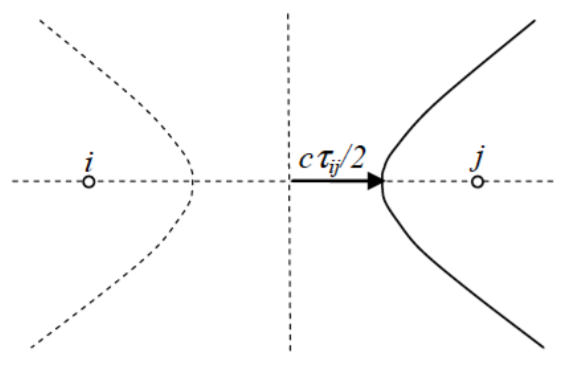
\includegraphics[width=0.4\textwidth]{figures/tdoa.png}
	\end{center}
	\caption{2D hyperbola loci defined for a TDOA of $\tau_{ij}$ between sensors $i$ and $j$}
	\label{fig:hyp}
\end{figure}

So, later on, with another pair of microphones, the intersection yields to the source localization.

In our short experiment, for tracking a minke whale on a 2D map, we have developed a rudimentary multilateration system, on the basis of 6 TDOAs only. The localization by itself leads to a non-linear solution. In addition, non-idealities imply a no unique solution, so we get a zone where the source could be located. We have not gone so far, but the estimated position could have been estimated by algorithms such as Crossing Lines or Steered-response power.

We first show the position of the hydrophones on the map, and then plot the hyperbolas corresponding to each pair of TDOA, assuming the speed of sound in water is 1510 m/s \cite{speed-sound-seawater}.  We have computed the TDOA between the sensor 1 and all the other ones, after having pre-processed the signals with PNR and doing the estimation with the Generalised Cross-Correlation Smoothed Coherence Transform.

\begin{figure*}[htb]
	\begin{center}
		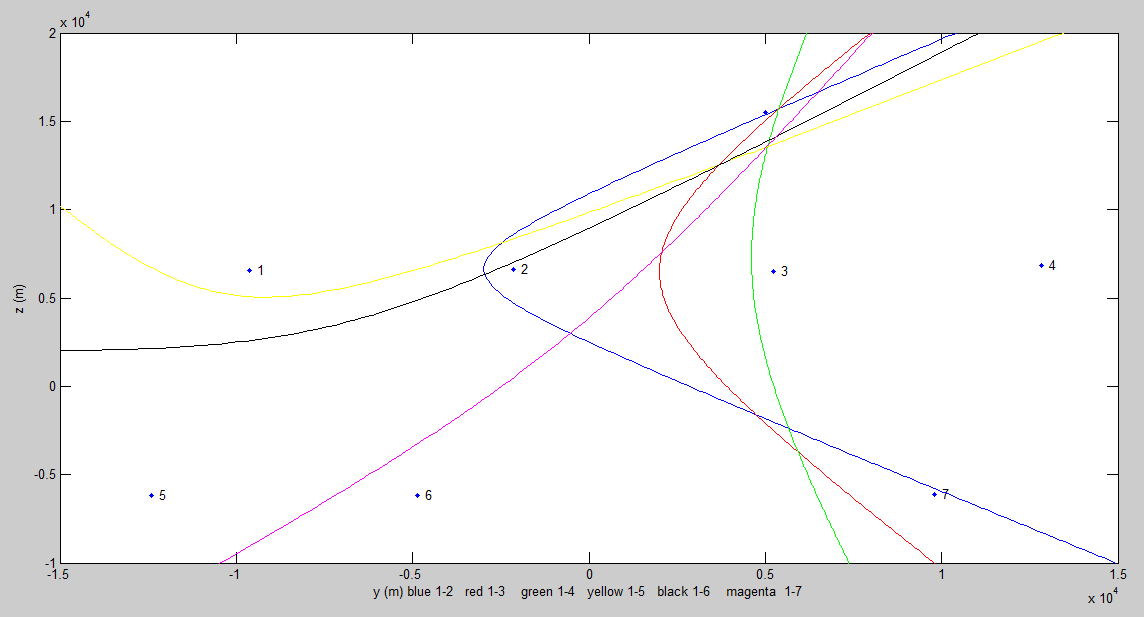
\includegraphics[width=1\textwidth]{figures/7_local.png}
	\end{center}
	\caption{Localization of the minke whale through multilateratization between sensor 1 and the rest.}
	\label{fig:local}
\end{figure*}

Then, looking at Figure \ref{fig:local}, we have obtained 7 curves that ideally will intersect at one point. In our case, it is quite normal that the curves don't intersect all, but we can see where the whale is approximately, as the curves intersect in a little area. The first 5 curves have a Time Delay Estimation error smaller than 1\%. The worst case corresponds to the furthest sensors, 1 and 7, and they are separated \SI{28}{\kilo\meter}, so our resolution is \SI{280}{\meter}. That is why the curves don't match in one point. Nevertheless, we do a rough visual estimation so the whale is at the position x=13700 y=5300.
